\documentclass[9pt]{beamer}
\mode<presentation>

% Theme choice:
\usetheme{Madrid}%Darmstadt 

\usecolortheme[RGB={0,100,50}]{structure}
 \usefonttheme{structurebold} 
\setbeamercovered{invisible}
%\setbeamertemplate{navigation symbols}{}
\usepackage{dynblocks}
\usepackage{textpos}
\usepackage{amsfonts}
\usepackage{amsmath}
\usepackage{amssymb}
\usepackage{amsthm}

\newtheorem{teorema}{Teorema}\usepackage{mathtools}
\renewcommand{\proofname}{Prova}
\usepackage[portuguese]{babel}

\uselanguage{Portuguese}
\languagepath{Portuguese}

\deftranslation[to=Portuguese]{Theorem}{Teorema}
\deftranslation[to=Portuguese]{Lemma}{Lema}
\deftranslation[to=Portuguese]{Corollary}{Corolário}
\deftranslation[to=Portuguese]{Proof}{Prova}

\usepackage{dutchcal}
\usepackage{hyperref}
\usepackage[utf8]{inputenc}
\usepackage[T1]{fontenc}
\usepackage{amsthm}


\usepackage[affil-it]{authblk} 
\usepackage{etoolbox}
\usepackage{lmodern}

\makeatletter
\patchcmd{\@maketitle}{\LARGE \@title}{\fontsize{18}{19.2}\selectfont\@title}{}{}
\makeatother

\renewcommand\Authfont{\fontsize{12}{14.4}\selectfont}
\renewcommand\Affilfont{\fontsize{9}{10.8}\itshape}

% Title page details: 
\title[Presentation]{Banco de Dados} %add title


\institute[UniRV]{\textbf{\large  \textcolor{structure}{\textbf{\large
Uma introdução.
}} %add name 
% \hspace{0.5pt}
\\ \qquad
\\Professor: Me. Sergio Souza Novak 
\\Faculdade de Engenharia de Software}
} 
% \titlegraphic{
\includegraphics[width=5cm]{msu.eps}}
\titlegraphic{
\includegraphics[width=5cm]{Universidade_de_Rio_Verde.jpg}}
\date{}

% Logo only on title page
%\logo{
\includegraphics[width=1cm,keepaspectratio]{Logo.png}}
\usepackage[pscoord]{eso-pic}


\begin{document}

% Title page frame
%\begin{frame}
    %\titlepage 
%\end{frame}
\frame[plain]{\titlepage}
%logo
\AddToShipoutPictureFG{
    \put(\LenToUnit{.92\paperwidth},
    \LenToUnit{.185\paperheight})
    {\vtop{{\null}
    \makebox{
\includegraphics[width=.8cm,keepaspectratio]{Universidade_de_Rio_Verde.jpg}}}}}


\begin{frame}{Sumário}
  \tableofcontents
\end{frame}
\section{Contextualização}


\begin{frame}{Bancos de Dados e Usuários de Banco de Dados}

Bancos de dados e sistemas de banco de dados são componentes essenciais da
sociedade moderna. Grande parte das atividades cotidianas envolve, direta ou
indiretamente, a interação com algum banco de dados.

\vspace{0.3cm}

\begin{itemize}
    \item Operações bancárias (depósitos, saques, transferências);
    \pause
    \item Reservas de hotéis e passagens aéreas;
    \pause
    \item Consultas a catálogos de bibliotecas;
    \pause
    \item Compras on-line (livros, eletrônicos, brinquedos);
    \pause
    \item Controle automático de estoque em supermercados.
\end{itemize}

\vspace{0.3cm}

Essas aplicações são exemplos de \textbf{aplicações tradicionais de bancos de dados},
nas quais os dados armazenados são predominantemente \textbf{textuais ou numéricos}.

\end{frame}
% Slide 1 — Redes sociais e novos tipos de dados
\begin{frame}{Redes Sociais e Bancos de Dados em Larga Escala}

\begin{block}{Proliferação de redes sociais}
A proliferação de websites de redes sociais, como Facebook, Twitter e Flickr,
exigiu a criação de bancos de dados imensos, capazes de armazenar grandes
volumes de dados não tradicionais.
\end{block}

\begin{block}{Tipos de dados armazenados}
Esses sistemas lidam com dados como postagens, tuítes, imagens e clipes de
vídeo, que apresentam alto volume, variedade e velocidade de geração.
\end{block}

\end{frame}

% Slide 2 — Big Data, NoSQL e grandes empresas
\begin{frame}{Big Data e Sistemas NoSQL}

\begin{block}{Sistemas Big Data e NoSQL}
Para atender às demandas das aplicações de mídia social, surgiram novos
tipos de sistemas de banco de dados, conhecidos como sistemas de
armazenamento \textbf{Big Data} ou sistemas \textbf{NoSQL}.
\end{block}
 \begin{figure}[H]
        \centering
        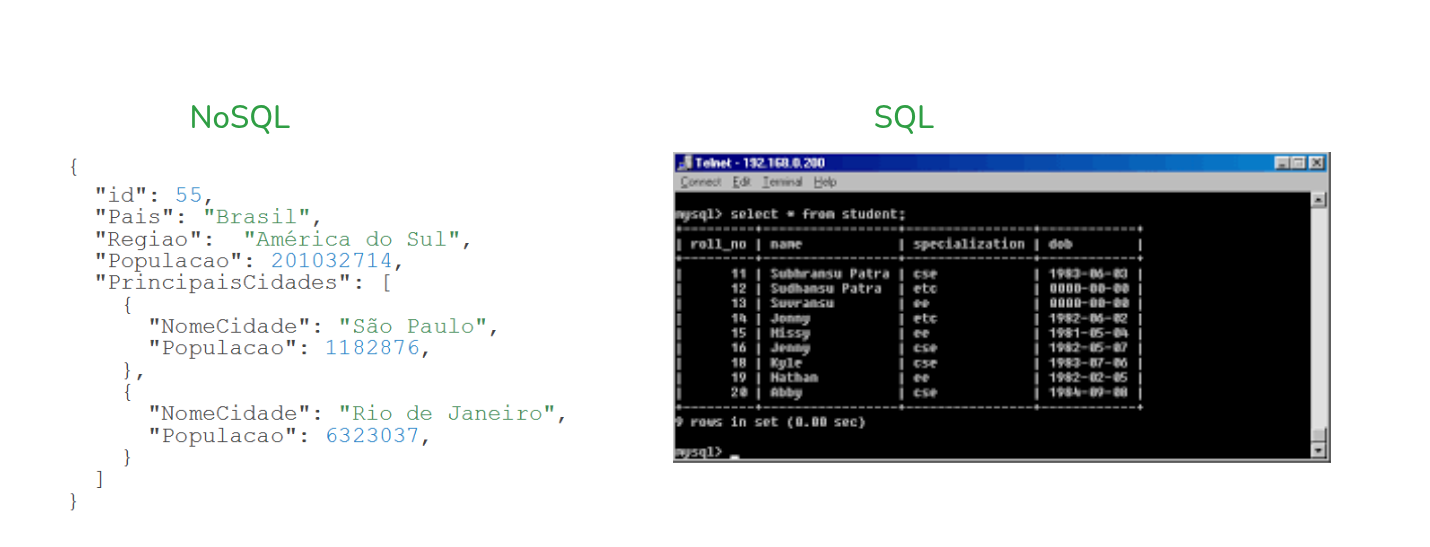
\includegraphics[width = 15cm]{comparacao_db.png}
    \end{figure}
\end{frame} 

\begin{frame}{Usos em grandes empresas}
        \begin{figure}
        \centering
        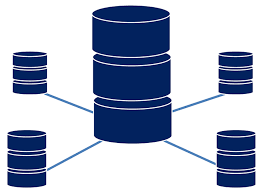
\includegraphics[width = 5cm]{multipledb.png}
    \end{figure}
\begin{block}{Uso em grandes empresas}
Esses sistemas são amplamente utilizados por empresas como Google,
Amazon e Yahoo para gerenciar dados de mecanismos de busca e serviços
de armazenamento em nuvem.
\end{block}

\end{frame}

% Slide 3 — Armazenamento em nuvem e multimídia
\begin{frame}{Armazenamento em Nuvem e Bancos Multimídia}
 \begin{figure}[H]
        \centering
        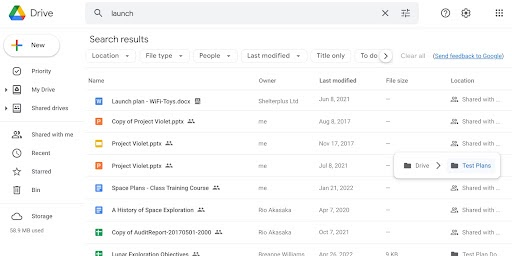
\includegraphics[width = 5cm]{gdrive.jpeg}
    \end{figure}
\begin{block}{Armazenamento em nuvem}
O armazenamento em nuvem permite que usuários gerenciem diversos tipos
de dados na web, incluindo documentos, programas, imagens, vídeos e
e-mails.
\end{block}

\begin{block}{Bancos de dados multimídia}
A ampla disponibilidade de tecnologias de foto, áudio e vídeo em dispositivos
móveis tornou comum o armazenamento digital de imagens, clipes de áudio
e streams de vídeo em bancos de dados multimídia.
\end{block}

\end{frame}
% Slide 4 — Outras aplicações modernas de bancos de dados
\begin{frame}{Outras Aplicações de Bancos de Dados}
 \begin{figure}[H]
        \centering
        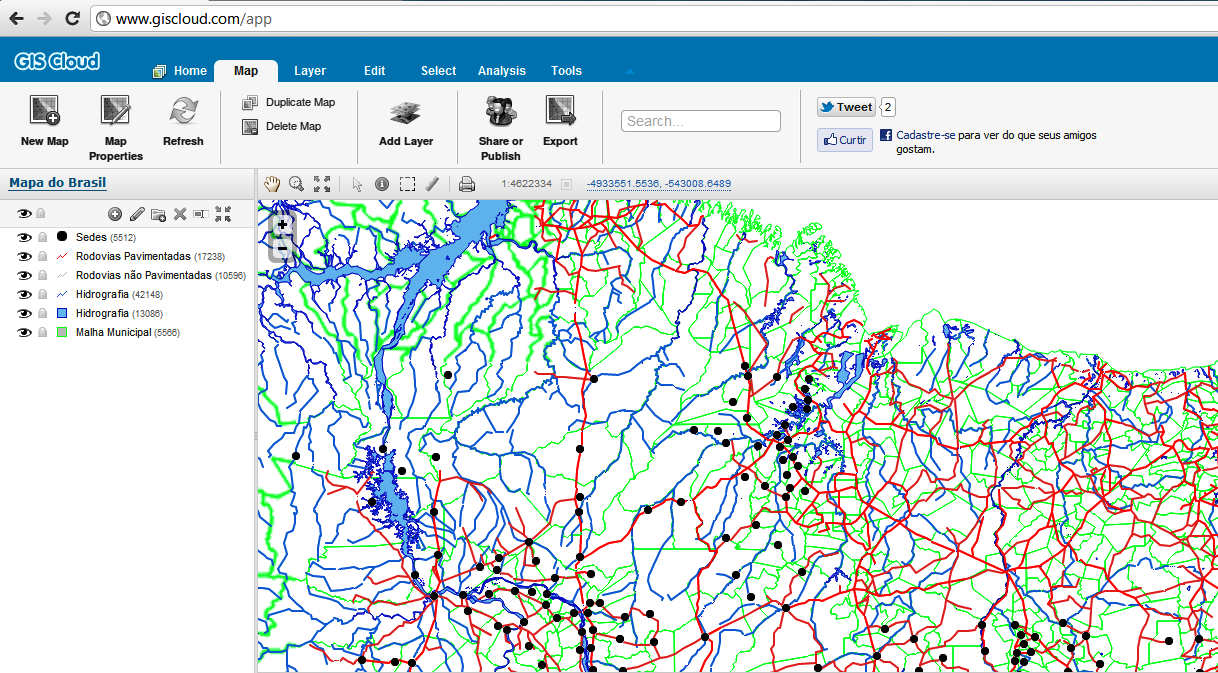
\includegraphics[width = 8cm]{giscloud1.png}
    \end{figure}
\begin{block}{GIS e análise espacial}
Sistemas de Informações Geográficas (GIS) armazenam e analisam mapas,
dados climáticos e imagens de satélite.
\end{block}

\begin{block}{Data Warehousing e OLAP}
Sistemas de Data Warehousing e Processamento Analítico On-Line (OLAP)
são usados para extrair e analisar grandes volumes de dados, apoiando a
tomada de decisão empresarial.
\end{block}

\begin{block}{Tempo real e Web}
Tecnologias de bancos de dados em tempo real e bancos de dados ativos
controlam processos industriais. Técnicas de pesquisa em bancos de dados
também são aplicadas à Web para melhorar a busca por informações.
\end{block}

\end{frame}

\section{SGDB}

% Slide 1 — O que é um SGBD
\begin{frame}{O que é um SGBD?}
    \begin{figure}[H]
        \centering
        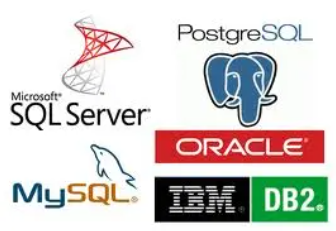
\includegraphics[width = 6cm]{sgdbs.png}
    \end{figure}
\begin{block}{Definição}
Um \textbf{Sistema Gerenciador de Banco de Dados (SGBD)} é um software
responsável por criar, armazenar, organizar e gerenciar bancos de dados,
permitindo o acesso eficiente, seguro e controlado às informações.
\end{block}

\begin{block}{Objetivo principal}
O SGBD atua como uma camada intermediária entre os dados armazenados e
as aplicações ou usuários que necessitam acessá-los.
\end{block}
 
\end{frame}
\begin{frame}{Visualização esquematica de um SGBD }

 \begin{figure}[H]
        \centering
        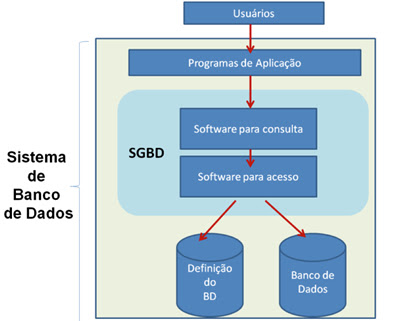
\includegraphics[width = 8cm]{unnamed.jpg}
    \end{figure}
\end{frame}

% Slide 2 — Funções fundamentais de um SGBD
\begin{frame}{Principais Funções de um SGBD}
    \begin{figure}
        \centering
        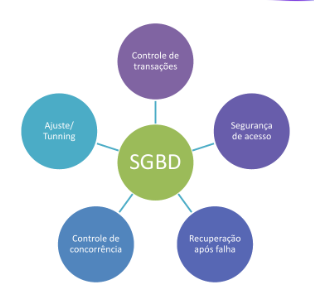
\includegraphics[width = 4cm]{funcoes_sgdb.png}
    \end{figure}
\begin{block}{Gerenciamento dos dados}
\begin{itemize}
    \item Armazenamento estruturado dos dados;
    \item Processamento eficiente de consultas;
    \item Manutenção da integridade e consistência das informações.
\end{itemize}
\end{block}

\begin{block}{Controle e segurança}
\begin{itemize}
    \item Controle de acesso e autorização de usuários;
    \item Controle de concorrência;
    \item Recuperação de falhas e suporte a backup.
\end{itemize}
\end{block}

\end{frame}
% Slide 3 — Importância do SGBD
\begin{frame}{Por que Utilizar um SGBD?}

\begin{block}{Vantagens}
O uso de um SGBD evita a manipulação direta de arquivos e reduz problemas
como redundância de dados, inconsistências, baixo desempenho e falhas
de disponibilidade.
\end{block}

\begin{block}{Contexto prático}
SGBDs são essenciais em aplicações modernas, desde sistemas locais até
grandes sistemas corporativos, web e ambientes de Big Data.
\end{block}

\end{frame}
\section{Estudo de caso sem uso de SGBD}

% Slide 1 — O problema real
\begin{frame}{Um Caso Prático: Sistema sem Banco de Dados}
    \begin{figure}[H]
        \centering
        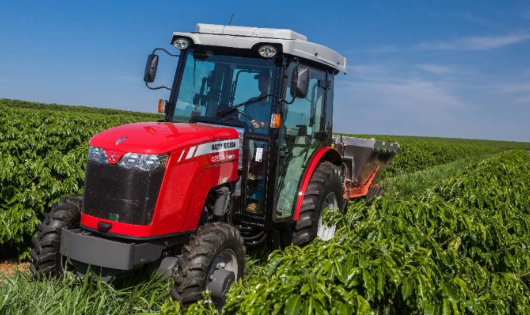
\includegraphics[width = 6cm]{trator.png}
    \end{figure}

\begin{block}{Contexto do projeto}
Um estudante, Ivan, decidiu implementar uma aplicação local em seu Trabalho
de Conclusão de Curso para gerenciar dados de um sistema de ponto de tratores
em uma fazenda.
\end{block}

\begin{block}{Decisão de projeto}
A aplicação não utilizava um Sistema Gerenciador de Banco de Dados (SGBD),
armazenando e manipulando diretamente arquivos do sistema operacional.
\end{block}

\end{frame}





% Slide 2 — Problemas enfrentados
\begin{frame}{Problemas Observados na Aplicação}
 \begin{figure}[H]
        \centering
        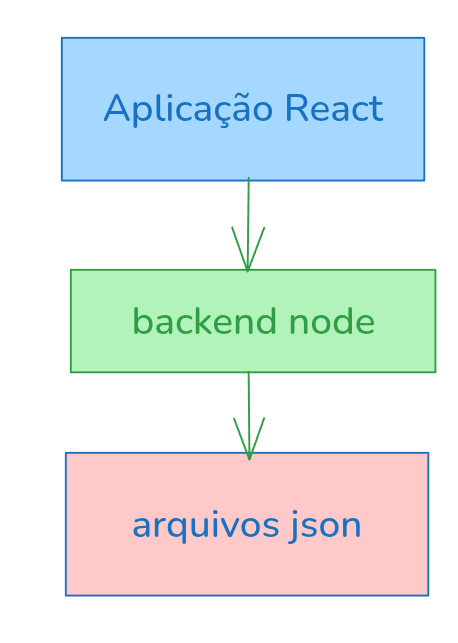
\includegraphics[width = 3cm]{fail.png}
    \end{figure}

\begin{block}{Disponibilidade e desempenho}
O sistema apresentava quedas frequentes, ficava fora do ar e realizava
consultas muito lentas, especialmente à medida que o volume de dados crescia.
\end{block}

\begin{block}{Confiabilidade dos dados}
Não havia mecanismos de backup ou redundância, tornando os dados vulneráveis
a falhas, perdas acidentais ou corrupção de arquivos.
\end{block}

\end{frame}
% Slide 3 — Reinventando a roda
\begin{frame}{Reinventando a Roda}
 \begin{figure}[H]
        \centering
        
\includegraphics[width = 5cm]{images.jpeg}
    \end{figure}

\begin{block}{Ausência de funcionalidades essenciais}
Ao não utilizar um SGBD, funcionalidades clássicas como controle de
concorrência, recuperação de falhas, integridade dos dados e segurança
precisaram ser implementadas manualmente — de forma incompleta.
\end{block}

\begin{block}{Lição aprendida}
Esse cenário é um exemplo clássico de \textbf{reinvenção da roda}, onde
soluções já consolidadas na área de bancos de dados deixam de ser aproveitadas.
\end{block}

\end{frame}
% Slide 4 — Conexão com conceitos introdutórios
\begin{frame}{Conexão com Bancos de Dados}

\begin{block}{Por que usar um SGBD?}
Sistemas de banco de dados existem para garantir:
\begin{itemize}
    \item Eficiência em consultas;
    \item Alta disponibilidade e confiabilidade;
    \item Backup e recuperação de falhas;
    \item Escalabilidade e integridade dos dados.
\end{itemize}
\end{block}


\begin{block}{Motivação para o estudo}
Casos como o do Ivan mostram a importância dos conceitos introdutórios de
bancos de dados e justificam o uso de SGBDs mesmo em aplicações locais.
\end{block}

\end{frame}
\section{Requisitos de um Sistema de Banco de Dados}

\begin{frame}{Requisitos e Propriedades de um Banco de Dados}
    \begin{table}
        \centering
        \caption{Principais Requisitos de Sistema e Consistência}
        \renewcommand{\arraystretch}{1.2}
        \begin{tabular}{|l|p{6cm}|} % Diminuí para 6cm para evitar Overfull hbox
            \hline
            \textbf{Requisito} & \textbf{Descrição} \\ \hline
            Confiabilidade & Manter dados precisos e acessíveis sob falhas. \\ \hline
            Integridade    & Segue regras (chaves primárias, tipos). \\ \hline
            Segurança      & Controle de acesso e autorizações. \\ \hline
            Desempenho     & Eficiência e tempo de resposta rápido. \\ \hline
            Escalabilidade & Suporte ao crescimento de dados/usuários. \\ \hline
            ACID           & Atomicidade, Consistência, Isolamento e Durabilidade. \\ \hline
        \end{tabular}
    \end{table}
\end{frame}
\section{Estudo de caso do CNJ}

\begin{frame}{Estudo de Caso}
    \begin{columns}[c] % [c] centraliza o conteúdo das colunas verticalmente
        
        \begin{column}{0.30\textwidth}
            \begin{figure}
                \centering
                
\includegraphics[width=\textwidth, height=0.4\textheight, keepaspectratio]{ministro.jpg}
                \caption{Alexandre de Moraes, ministro do STF.}
            \end{figure}
        \end{column}

        \begin{column}{0.30\textwidth}
            \begin{figure}
                \centering
                
\includegraphics[width=\textwidth, height=0.4\textheight, keepaspectratio]{walter.jpeg}
                \caption{Walter Delgatti Neto.}
            \end{figure}
        \end{column}

        \begin{column}{0.30\textwidth}
            \begin{figure}
                \centering
                
\includegraphics[width=\textwidth, height=0.4\textheight, keepaspectratio]{carla.jpeg}
                \caption{Carla Zambelli.}
            \end{figure}
        \end{column}
        
    \end{columns}
\end{frame}
\begin{frame}{Mandado de Prisão Falso Contra Alexandre de Moraes}
Durante a invasão ao sistema do Conselho Nacional de Justiça (CNJ), em 2023, o hacker
\textbf{Walter Delgatti Neto} inseriu documentos fraudulentos no Banco Nacional de
Mandados de Prisão (BNMP).

\begin{itemize}
  \item Entre os documentos falsos estava um \textbf{mandado de prisão contra o ministro Alexandre de Moraes}, do Supremo Tribunal Federal (STF).
  
  \item O texto do mandado afirmava, de forma fraudulenta:
  \begin{quote}
  ``Expeça-se mandado de prisão em desfavor de mim mesmo, Alexandre de Moraes.''
  \end{quote}
  Ou seja, um mandado que simulava ter sido expedido pelo próprio ministro contra si mesmo.
  
  \item Segundo as investigações, o objetivo da ação era desmoralizar o Poder Judiciário e comprometer a credibilidade dos sistemas institucionais.
\end{itemize}
\end{frame}
\begin{frame}{Requisitos de um SGBD e o Caso do CNJ}
O caso da invasão ao sistema do Conselho Nacional de Justiça (CNJ) evidencia falhas
críticas em requisitos fundamentais de um Sistema Gerenciador de Banco de Dados (SGBD),
especialmente em sistemas de missão crítica e alta sensibilidade institucional.
\end{frame}
\begin{frame}{Segurança e Controle de Acesso}
\begin{itemize}
  \item \textbf{Segurança}: houve acesso não autorizado ao banco de dados do sistema judicial.
  \item \textbf{Autenticação}: credenciais válidas foram utilizadas de forma indevida.
  \item \textbf{Autorização}: o sistema permitiu operações além do escopo funcional do usuário.
  \item \textbf{Violação do princípio do menor privilégio}.
\end{itemize}

Essas falhas permitiram a inserção de registros judiciais falsos no banco de dados.
\end{frame}
\begin{frame}{Segurança e Controle de Acesso}
\begin{itemize}
  \item \textbf{Segurança}: houve acesso não autorizado ao banco de dados do sistema judicial.
  \item \textbf{Autenticação}: credenciais válidas foram utilizadas de forma indevida.
  \item \textbf{Autorização}: o sistema permitiu operações além do escopo funcional do usuário.
  \item \textbf{Violação do princípio do menor privilégio}.
\end{itemize}

Essas falhas permitiram a inserção de registros judiciais falsos no banco de dados.
\end{frame}
\begin{frame}{Integridade e Consistência dos Dados}
\begin{itemize}
  \item \textbf{Integridade}: o SGBD aceitou dados semanticamente inválidos
  (mandado de prisão inexistente).
  \item \textbf{Integridade semântica}: ausência de validação das regras de negócio.
  \item \textbf{Consistência}: o banco entrou em um estado inconsistente,
  violando o princípio de consistência das transações (ACID).
\end{itemize}

Um registro judicial não correspondia a nenhum processo ou decisão válida.
\end{frame}
\begin{frame}{Auditoria, Confiabilidade e Disponibilidade}
\begin{itemize}
  \item \textbf{Auditoria}: falha na detecção imediata de operações anômalas.
  \item \textbf{Rastreabilidade}: ausência de bloqueios automáticos para ações críticas.
  \item \textbf{Confiabilidade}: comprometimento da confiança institucional nos dados.
  \item \textbf{Disponibilidade lógica}: o sistema permaneceu ativo, porém com dados não confiáveis.
\end{itemize}

Em sistemas críticos, dados incorretos equivalem à indisponibilidade do serviço.
\end{frame}



\begin{frame}{Aspectos Jurídicos e Consequências}
Do ponto de vista jurídico, Delgatti foi responsabilizado por crimes previstos no Código Penal e na legislação penal especial:

\begin{itemize}
  \item \textbf{Invasão de dispositivo informático} (art. 154-A do Código Penal);
  \item \textbf{Falsidade ideológica}, no caso da inserção de informações falsas em sistemas oficiais;
  \item Condenações impostas pelo STF e pela Justiça Federal, com penas privativas de liberdade.
\end{itemize}

O caso também envolveu a deputada federal Carla Zambelli, acusada de participação intelectual nos fatos, reforçando a dimensão política do episódio e sua relevância para o debate sobre responsabilidade penal no uso de tecnologias digitais.
\end{frame}


\begin{frame}{Bons estudos!}
    \begin{figure}
        \centering
        
\includegraphics[width = 9cm]{Universidade_de_Rio_Verde.jpg}
    \end{figure}
\end{frame}





\end{document}
